\chapter{时频传递的基本概念及进展}

高精度时间是现代生活、工业生产以及科学研究等领域的基石,而时频传递则是将高精度时钟应用于各种场景的关键技术,具有极其重要的价值。本章主要介绍时频传递的基本概念以及典型应用,并将时频传递中涉及到的几个关键评价指标进行了介绍。时频传递可以通过多种技术来实现,本章也介绍了目前几种主流的高精度时频传递技术,是为全文的研究背景。

\section{时频传递的基本概念}
\subsection{时频传递的概念及应用}
时频传递是将高精度时间频率信息进行准确的传递。因此它的主要研究内容是如何通过各种技术手段将高精度的时间频率信息进行传递,并尽可能地保证传递后的时间频率信息与传递之前的保持一致,即避免引入额外噪声而导致传递后的时间频率信息的不准确或性能恶化。这个过程涉及到两方面:首先存在一个被传递的时间频率源,其次通过技术手段将该时间频率信息进行传输并准确复现。从发展的历史来看,随着时间精度的不断提高,对时频传递的要求也将随之增加。

时间在现代物理学中是构成四维时空的一个维度,同时时间单位也是国际单位制(SI)的七个基本单位之一。如何衡量时间或者计时,一直是一个非常重要的问题,并且也与社会的科技水平直接相关。在古代社会中,人们最早是从天文现象来认识时间:太阳的日复一日的升起与降落导致出现天的概念,月亮的阴晴圆缺导致月份的概念,而四季物候变化和天象的斗转星移则导致了年的概念。在这个阶段,人们的计时手段完全依靠天象,并通过长期对天文的观测发展出了历法,例如古代中国的阴阳历,古埃及的太阴历,古罗马的儒略历等等。利用准确的历法能够指导农业生产,安排社会活动,但对于日常生活还需要更细致的计时方式。在小型化机械时钟出现之前,人们主要依靠日晷或者水钟等较为原始的方式来计时,将一天分为十二个时辰或二十四小时。这些计时方式精度不高,而且设备体型庞大,并不方便使用。在古代城市中,通常有一个钟楼位于城市中心区域,钟楼的作用即是通过敲击大钟进行报时,以便城市的民众知道目前的时间。该项行为实际上就是进行时间发布,通过声音信号将时间信息传递给能够听到的民众,虽然传递精度有限,但是已经能够满足当时社会的需求。随着十七八世纪小型化机械时钟的发展,特别是航海钟H4的出现,人们不仅可以随身携带精确的钟表,更进一步将准确的时间信息用于航海导航定位,极大推动了航海探索和社会发展。航海钟H4的历史很好的展现了一个时间比对的应用案例:在航海当中行船如何确定自己的经纬坐标在当时是一个难题,纬度可以通过太阳高度或北极星来很好确定,但经度却很难确定。当时有两种解决方案,一个是天文测算法,还有一个是时钟测算法。天文测试法需要进行大量的计算,对于航海应用并不实际,而时钟测算法原理比较简单:因为地球一天自转360度,则一小时转动对应的经度为十五度,即当地时钟起点与经度相关,如果有一块精确的时钟,在经度为0度的地点时调整时间与当地时钟一致,然后在航海中只需将时钟的时间与当地时间比较,其差别即可用来计算经度。哈里森发明了精确的H4航海钟从而解决了该难题,精确的时钟与对时在这里与导航定位联系了起来,其中时间比对采用的方式即为最普通但十分有效的搬运钟的形式。

随着科学技术的进一步发展,时钟越来越精确,从不确定度只有$10^{-6}$的机械时钟发展到$10^{-9}$的石英时钟,以及不确定度可达$10^{-12}$的原子钟。其中原子钟的发明不仅是技术上的突破,更是基础物理的发展,特别是量子力学为其提供了理论基础,才使得人类首次拥有如此精确的时钟。而目前国际单位的秒定义也与原子钟相关:单位秒是海平面上铯133($Cs^{133}$)原子基态的两个超精细能阶之间跃迁时所辐射的电磁波的周期的9,192,631,770倍的时间。在这里,稳定的频率和精确的时间是可以转化的。一个稳定的频率体系相当于提供了一个走速均匀的时钟,在此基础上我们只需定义一个时间起点,即可以得到一个时间体系。像国际原子时(TAI)、协调世界时(UTC)、GPS时等时间体系都是根据该方式并结合具体情况来定义的,它们在不同的领域有各自的应用。有了高精度时钟,对高精度的时频传递的要求也大大增加,为此人们发展了基于微波技术以及激光技术的时频传递,在此基础上高精度时间频率系统广泛应用于工业生活科学研究等方方面面,极大促进了社会的发展。

全球定位系统(GPS)就是一个非常成功的时间频率体系。它主要由GPS卫星星座、地面监控系统、用户系统三部分组成。GPS卫星携带了高精度的原子钟,并可以向用户播发用于导航定位的测距信息和导航电文,监控系统用于测定GPS卫星状态,上注指令等,用户接收GPS信号即可确定自己的位置和时间。在该系统中,时频传递占据了非常重要的地位。每颗GPS卫星代表一个精确的时钟,GPS星座维持了一个时频网络,并不断播发自己的时频信息,用户只需接收4颗及以上卫星的信号,分别与它们比对时间,由于卫星位置从导航电文中可以获得,根据信号传播的延时关系即可计算用户的位置以及真实时间。其中时频传递所依赖的技术即为微波技术,通过调制的微波信号将时间信息传递到用户所在地。目前GPS系统的授时精度可达几十纳秒,定位精度可到米级,完全改变了人们获取精确时间的方式,使得人类在地球任何地方都能极其方便并准确地知道自己的位置,同时也对许多科学领域,例如导航、地球物理、精密测量、航空航天等领域产生了巨大影响。在日常生活领域,准确的时间同步也扮演了非常重要的角色:通信网络、股票交易、广播电视等,它们都需要高精度的时间同步作为基础,其精度一般需要微秒或毫秒量级,如果时间发生错误,将会导致网络瘫痪,带来灾难性的影响。而在科学研究领域,精密时钟和时频传递是许多精密测量实验的基础,其精度要求更高。在相对论理论中,运动和重力场都会对时钟的走速产生影响,因此比较一个静止的和一个运动的时钟,或者比较不同重力场下的时钟都可以对相对论理论进行检验,例如引力红移、基础常数的时变特性、局域不变原理等等。而在深空探测器和遥感卫星上,精密时频及传递可以为它们提供导航定位以及用于遥感测绘等。目前冷原子钟的不确定度已经到$10^{-16}$的级别,并且即将应用于空间实验,而实验室中最先进的光钟的不确定度甚至可到$10^{-18}$,将成为未来秒定义的备选。这些新进展对于精密测量以及基础物理可谓意义重大,同时也对时频传递提出了更高的要求。

\subsection{时频传递的评价指标}
评价一种时频传递方法的性能涉及到测量以及噪声分析,因此在这里需要先提到关于测量及噪声的一些概念,例如精度、准确度、精确度、噪声以及稳定度等。

\textbf{精度(Precision):}用于描述多次测量结果之间的符合程度,在同样测试条件下多次测量得到的结果具有一定分布,这个分布可以用标准差(Standard Deviation)来刻画,表现了测量随机误差的大小。精度越高,则该标准差越小,说明测量值的随机误差越小。

\textbf{准确度(Trueness):}用于描述大量测试结果的平均值与被测对象的参考值之间的符合程度,可以用偏置(Bias)来刻画,表现了系统误差的大小。准确度越高,则偏置越小,测量平均值的系统误差越小。
\begin{figure}[htbp]
\centering
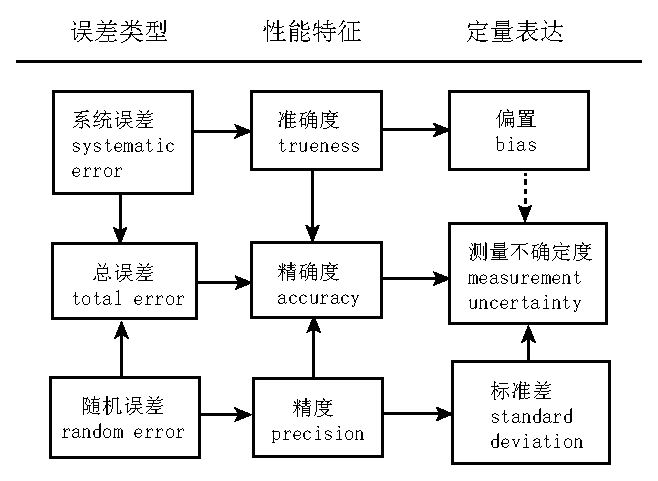
\includegraphics[width=.6\textwidth]{2-1-2-relationship}
\caption{误差以及精度等概念之间的关系}
\label{fig:2-1-2-relationship}
\end{figure}

\begin{figure}[htbp]
\centering
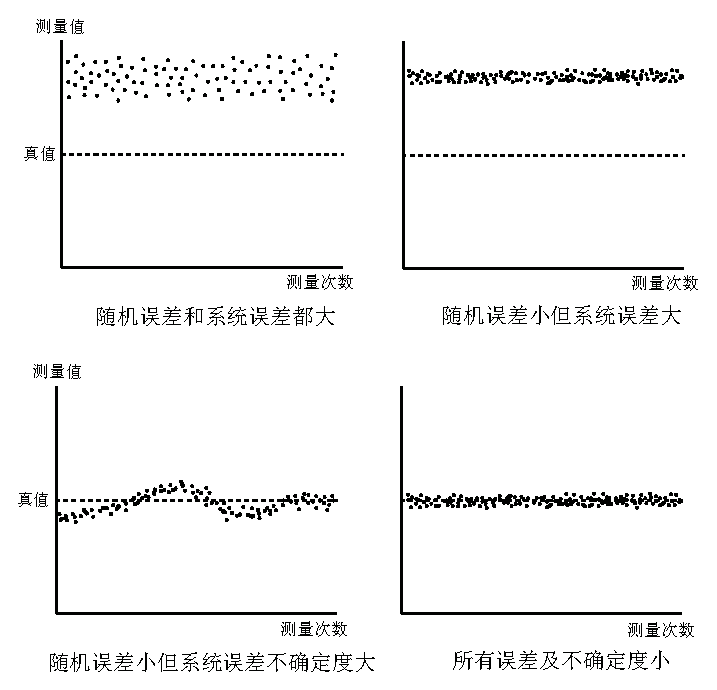
\includegraphics[width=.6\textwidth]{2-1-2-measurement}
\caption{几种典型的测量结果}
\label{fig:2-1-2-measurement}
\end{figure}

\textbf{精确度(Accuracy):}用于描述测量值与被测量对象的真值之间的符合程度,它包含了测量系统误差和随机误差两部分。衡量精确度的可信性是用测量不确定度(Measurement Uncertainty)来表示,通常写成标准差(标准不确定度)的形式,该不确定度包含了对系统误差估计的不确定度以及测量随机误差。

图 \ref {fig:2-1-2-relationship}给出了它们之间的关系,图\ref{fig:2-1-2-measurement}则画出了测量结果的几种典型案例。

\textbf{噪声:}在时频领域,噪声用来统指影响时间频率信号稳定度的所有因素。时钟产生的信号不是绝对稳定的,本身也存在噪声,而信号在传输过程中可能还会引入其它噪声。以正弦波输出的频率源为例,其形式为:
\begin{equation}
V(t)=[V_{0}+\varepsilon(t)]\sin [2\pi f_{0}t+\varphi(t)]
\end{equation}
其中,$V_{0}$,$f_{0}$分别为标称振幅和标称频率,$\varepsilon(t)$,$\varphi(t)$分别为振幅变化和相位变化。噪声即由各种因素带来的相位扰动,体现在$\varphi(t)$这一项。我们用$y(t)$来表示相对标称频率的归一化瞬时频率偏差:
\begin{equation}
y(t)\equiv\dfrac{\diff f(t)}{f_{0}}\equiv\dfrac{\dot{\varphi}(t)}{2\pi f_{0}}
\end{equation}
同理,在时域方面可以得到瞬时相对时间偏差$x(t)$:
\begin{equation}
x(t) \equiv \dfrac{\varphi(t)}{2\pi f_{0}}
\end{equation}
一般频率源的随机噪声过程可以用幂律谱模型来表征:
\begin{equation}
S_{y}(f)=h_{\alpha}f^{\alpha}
\end{equation}
其中,$f$为傅里叶频率,$S_{y}(f)$表示相对频率偏移谱密度,$h_{\alpha}$为幅度,$\alpha$为幂律谱指数。通常有五种独立噪声过程($\alpha=-2,-1,0,1,2$):频率随机游走噪声、调频闪烁噪声、调频白噪声、调相闪烁噪声和调相白噪声。

\textbf{稳定度(Stability):}在时频领域,用于描述在一定时间内,信号保持同样时间或频率的能力。它不能说明时间或频率是否准确,而是表明是否是同一个值。图\ref{2-1-2-stability}画出了信号的稳定度和准确度之间的关系。
\begin{figure}[htbp]
\centering
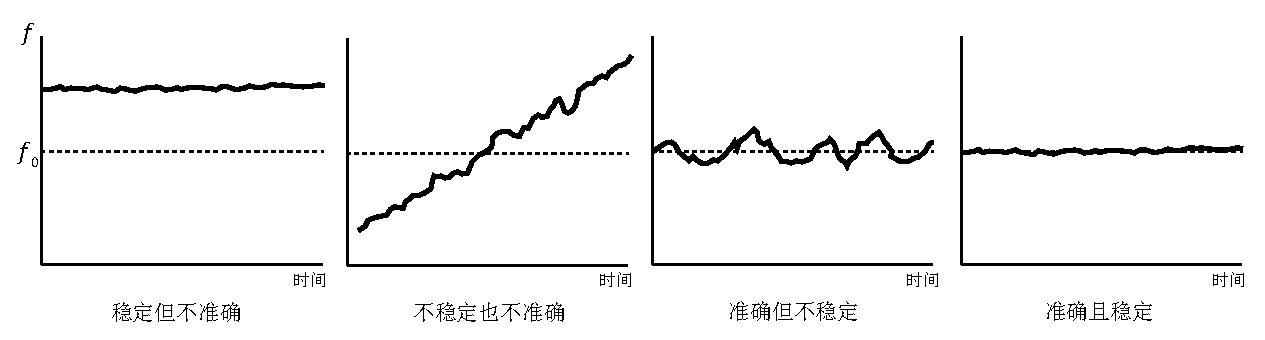
\includegraphics[width=.9\textwidth]{2-1-2-stability}
\caption{准确度与稳定度的关系}
\label{2-1-2-stability}
\end{figure}

从统计学上来说,稳定度是表征信号在给定时间段内频率偏差或相位偏差相对于平均频率偏差或平均相位偏差的波动。它可以在时域测量,即获得相位(时间)偏差数据,或者在频域测量,即获得频率偏差数据,利用这些数据可以计算其统计特性。一般标准方差只对平稳数据有效,对于平稳数据过程,统计特征与时间独立,例如白噪声,其频带内为均匀分布的噪声。在这种过程中,均值与方差随着测量次数增加会收敛到同一个值。而对于非平稳数据,该过程包含了时变噪声,其均值和方差不会收敛到某一个值,平均值会滑动变化。因此我们需要采用新的统计方法来表征时间频率信号的稳定度。这里介绍几个常用的用于描述稳定度的统计方差:Allan方差、修正Allan方差,以及时间方差。由于在通常使用中,一般取其平方根即偏差来表述,因此下文直接介绍偏差的定义。

\textbf{Allan偏差(ADEV):}传统的标准方差对调频闪烁噪声和频率随机游走噪声不收敛,Barnes和Allan基于频率数据的一阶差分或者时差数据的二阶差分而得到了一种可以表征时间频率稳定度的收敛的方法,其计算公式如下:
\begin{equation}
\sigma_{y}(\tau)=\sqrt{\dfrac{1}{2(M-1)}\sum_{i=1}^{M-1}(y_{i+1}-y_{i})^{2}}
\end{equation}
其中,$y_{i}(i=1,2,\cdot\cdot\cdot,M)$是相对频率测量值,M是测量数据的个数,数据为等间隔测量。Allan偏差也可以通过相位(时间)测量数据来计算,计算公式如下:
\begin{equation}
\sigma_{y}(\tau)=\sqrt{\dfrac{1}{2(N-2)\tau^{2}}\sum_{i=1}^{N-1}(x_{i+2}-2x_{i+1}+x_{i})^{2}}
\end{equation}
其中,$x_{i}(i=1,2,\cdot\cdot\cdot,N)$是相位测量值,单位为时间单位,N为测量数据个数,其测量时间间隔为时间$\tau$。

\textbf{修正Allan偏差(MDEV):}相比于Allan偏差,该方式通过改变测量系统的带宽或者计算测量数据的谱来对不同类型噪声进行辨别,能更好的区分调相白噪声和调相闪烁噪声。其计算公式如下:
\begin{equation}
Mod\,\sigma_{y}(\tau)=\sqrt{\dfrac{1}{2\tau^{2}}[\dfrac{1}{m}\sum_{i=1}^{m}(x_{i+2m}-2x_{i+m}+x_{i})]^{2}}
\end{equation}
其中$\tau=m\tau_{0}$,$\tau_{0}$是数据测量时间间隔(硬件带宽),即软件带宽为硬件带宽的$1/m$,$x_{i}$是相位测量值。同理,MDEV也可以根据频率测量数据来计算,这里不再介绍。

\textbf{时间偏差(TDEV):}Allan偏差和修正Allan偏差比较适合进行频率测量来表征频率标准的频率稳定度的情况,而对于采用时间测量来计算时间稳定度的情况,则更适合采用时间偏差来表征,它是在修正Allan偏差的基础进行了改进,其形式如下:
\begin{equation}
\sigma_{x}(\tau)=\dfrac{1}{\sqrt{3}}\tau Mod\,\sigma_{y}(\tau)
\end{equation}

在时频传递中,有的方案只传递频率信号,有的只传递时间脉冲信号,也有的方案两者都能传递。频率传递重点在于使得两地时钟的走速可以比较,进而可以对从钟的走速进行调整即实现频率同步。时间传递在于可以比对两地时钟的时刻,使得从钟的时间与主钟的相位同步。两者存在一定差异,值得注意的是时间传递也能够用来比对频率,即通过时间换算可测频率关系。无论是频率传递还是时间传递,其性能评价一般关注的是传递不确定度以及稳定度。传递不确定度关注的信号传递的精确性,而稳定度关注的是传递过程中带来额外噪声的程度。

\section{几种主要的时频传递}
随着高精度时钟的发展,时频传递也取得了很大的进步。目前高精度时频传递所采用的信号载体主要是微波和激光,其中激光又分为光纤以及自由空间两种应用场景。下面将分别介绍微波、光纤激光、自由空间激光三个技术路线的主要方案和进展。

\subsection{微波时频传递}
鉴于微波技术本身的成熟度,在信号调制、发射及接收等方面都非常方便,覆盖区域广阔,而且大部分高精度时钟输出的为微波信号,具有很好的兼容性,基于微波来进行时频传递已成为应用最为广泛的解决方案。目前主要的微波时频传递方案有:罗兰-C、GPS卫星共视、GPS载波相位、卫星双向时频传递等。本小节将以GPS卫星共视和卫星双向时频传递为代表,介绍其实现原理。

\paragraph*{GPS卫星共视时频传递}
上世纪八十年代初期随着GPS系统的初步建立,美国国家标准局的Allan和Weiss提出可以利用GPS卫星实现时频传递,该方案利用共视来星历以及大部分的链路共模误差,设备简单,取得了很好的效果。其主要原理如图\ref{2-2-1-CV}所示。处于不同地方的两个GPS接收机A,B分别都接收来自于同一个GPS卫星的信号,得到本地GPS信号的到达时间,通过修正信号传播延时来比较两地钟差。令A,B测得的GPS信号时间为$T_{A}$,$ T_{B}$,两边信号的传播延时为$\tau_{A}$,$\tau_{B}$,则两地钟差$\tau$可以写成如下公式:
\begin{equation}
\tau=(T_{A}-\tau_{A})-(T_{B}-\tau_{B})
\end{equation}
其中信号的传播延时包含了卫星到地面站的几何距离延时、电离层延时、对流层延时以及本地电子学等系统延时。
\begin{figure}[htbp]
\centering
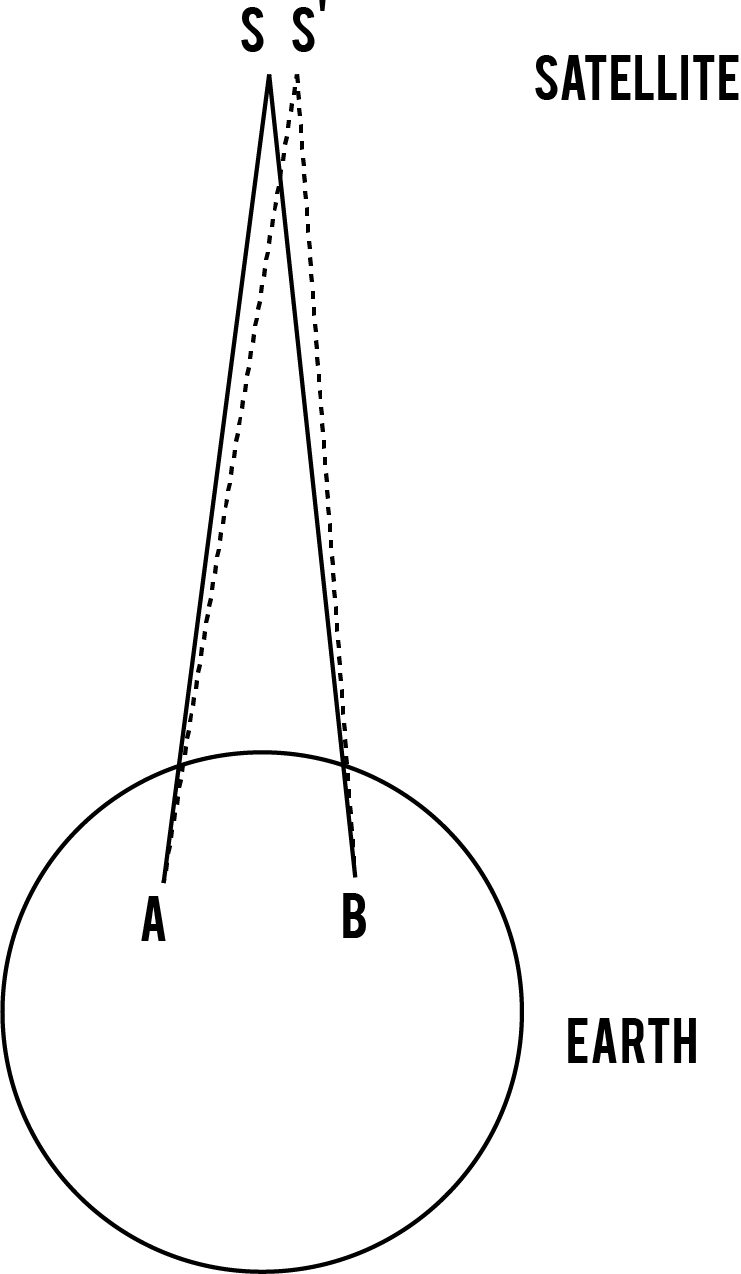
\includegraphics[width=.3\textwidth]{2-2-1-CV.png}
\caption{GPS卫星共视时频传递原理图}
\label{2-2-1-CV}
\end{figure}

几何延时可以根据GPS的星历进行估算,因此星历误差将会影响比对结果。在共视方案中,能够有效消除大部分星历,下面给出详细分析。假设地面接收机天线的位置坐标矢量分别为$\vec{A} ,\vec{B}$,卫星星历位置矢量为$\vec{S}$ ,而真实位置矢量为$\vec{S'}$。卫星位置误差则为:$\Delta S=\vec{S'}-\vec{S}$,在计算卫星到地面站的距离引入的误差则为:
\begin{subequations}
    \begin{align}
        \Delta r_{A}&=\vec{e_{A'}}\cdot \overrightarrow{S'A}-\vec{e_{A}}\cdot \overrightarrow{SA}\\
        \Delta r_{B}&=\vec{e_{B'}}\cdot \overrightarrow{S'B}-\vec{e_{B}}\cdot \overrightarrow{SB}
    \end{align}
\end{subequations}
其中$\vec{e_{A'}},\vec{e_{A}}$分别为由卫星位置$S',S$至地面站A矢量$\overrightarrow{S'A},\overrightarrow{SA}$的单位向量。由于它们的夹角非常小,在一阶近似下,$\vec{e_{A'}}=\vec{e_{A}}$,同理$\vec{e_{B'}}=\vec{e_{B}}$,代入上面公式可以得到:
$\Delta r_{A}=\vec{e_{A}} \cdot \Delta S,\Delta r_{B}=\vec{e_{B}} \cdot \Delta S$,则共视时卫星位置误差引入的时间比对误差为:
\begin{equation}
    \Delta \tau_{AB}=(\Delta r_{B}-\Delta r_{A})/c=\frac{1}{c}(\vec{e_{B}} -\vec{e_{A}} )\cdot \Delta S
\end{equation}
可以看出,当$\vec{e_{A}},\vec{e_{B}}$越接近平行时,也就是地面接收机A,B与卫星连线的夹角越小时,引入的误差$\Delta \tau_{AB}$越小。
该夹角与卫星轨道高度以及地面站A,B之间的距离(基线长度)有关。对于共视GPS卫星,基线长度在几千公里级别时能够消除约$90\%$以上的误差。一些详细的模拟计算案例可以见参考文献[...]。

电离层延时是微波信号在经过距地面约50公里以上的大气层时,由于该层大气有电离现象,信号受电子影响而产生的延时,其延时大小与信号所经过的路径上的总电子含量(TEC)有关:
\begin{equation}
\tau_{ion}=\dfrac{40.3\cdot TEC}{c f^{2}}
\end{equation}
其中$c$为光速,$f$为信号的频率。对于约1.5GHz的微波信号,电离层可能带来约几十纳秒的延时,信号频率越高,则该项影响越小。该项延时修正可以通过IGS(International GNSS Service)组织提供的电离层总电子含量图来计算,或者采用双频信号进行测量来消除电离层影响;此外,也可以通过模型修正,例如Klobuchar模型等。

对流层指从地面往上直到约$10\sim 20$公里左右的大气层,受重力影响,该层集中了约75\%的大气质量和90\%以上的水汽质量,其折射率随高度而发生变化。对于L波段($1\sim2GHz$)的电磁波,对流层延时与频率关系不大,因此不能采用双频信号来测量修正,一般依靠模型计算延时。对流层可以通过干燥以及潮湿两个分量来建模,干燥分量是由干燥空气引起的,带来约90\%的延迟量,能够精确建模;而潮湿分量主要是来源于空气中的水蒸气,相对来说不确定性要大一些。目前广泛使用的Hopfield模型的延时修正误差能到1ns左右。

在不太长的基线下,两地的电离层和对流层都有一定的相关性,共视能够消除一部分的共模误差。除以上延时修正之外,本地电子学延时例如线缆、电子学器件、天线相位中心等也需要进行标定修正。此外还需考虑测量时的多孔径效应以及地球自转带来的Sagnac效应。共视法由于设备简单,比对不确定度能达到几纳秒,日稳定度可达$10^{-15}$,自上世纪九十年代起就正式作为国际原子时(TAI)比对计算的主流方法。随着GPS技术的发展,后续还有全视法、载波相位等方法出现,具有一定的改善,在此不多做介绍。

\paragraph*{卫星双向时频传递}
由于共视法的信号传播链路为单向链路(one-way),非共模误差很难消除,为了进一步提高时频传递精度,人们提出了卫星双向时频传递(TWSTFT),通过卫星中转(一般为同步轨道卫星),两地相互发射与接收微波信号来进行时频传递。在TWSTFT中,双向链路(two-way)具有很好的共模性质,能够消除大部分的传播延时,因此比共视法具备更好的性能。其基本原理如图所示。令A地的信号发射与接收时间分别为$T_{AS}$,$T_{AR}$,B地的信号发射与接收时间为$T_{BS}$和$T_{BR}$,信号的传播延时分别为$\tau_{A \rightarrow B}$,$\tau_{B \rightarrow A}$,则两地钟差$\tau$可以通过以下公式计算:
\begin{equation}
\tau=\dfrac{1}{2}(T_{AR}-T_{BS}+T_{AS}-T_{BR}+\tau_{A \rightarrow B}-\tau_{B \rightarrow A})+S
\end{equation}
其中S为地球自转带来的Sagnac效应补偿项。传播延时包括了本地系统延时、卫星信号转发延时、几何路径延时、电离层以及对流层延时等。在双向传递中,信号的几何路径延时、电离层以及对流层延时基本一致,而本地系统延时、卫星信号转发延时都可以进行精确标定。因此TWSTFT的比对精度和稳定性都优于共视法,可以获得亚纳秒的比对不确定度以及$10^{-16}$的日稳定度。该方案也已经正式用于TAI的比对计算,是目前性能最优的远距离微波时频传递方案之一。

\subsection{光纤激光时频传递}

\subsection{自由空间激光时频传递}
